\documentclass{beamer}
\usepackage{beamerthemesplit}
\usepackage{graphicx,url}
\usepackage[brazil]{babel}
\usepackage[utf8]{inputenc}
\usepackage{multimedia}

\mode<presentation>
{
  \usetheme{Ilmenau}
  \setbeamercovered{transparent}
}

\newcommand{\eng}[1]{\textit{#1}}
\newcommand{\obra}{\textit{Em torno da romã}}
\newcommand{\goiaba}{\textit{Goiaba}}
\newcommand{\redmark}[1]{\textcolor{red}{#1}}
\newcommand{\graymark}[1]{\textcolor{gray}{#1}}
\newcommand{\tocar}{\textcolor{blue}{$\blacktriangleright$}}

\title{\obra{}: aplicações de operações de contorno na composição---Anexo}
\author{Marcos da Silva Sampaio}
\date{28 de novembro de 2008}

\logo{\includegraphics[scale=.15]{logo-genos}}

\begin{document}
\frame{
  \frametitle{Possível coerência em Webern}
\begin{figure}
  \centering
    \includegraphics[scale=.7]{webern-tema-analisado}

    \includegraphics[scale=.7]{webern-concatenacao-1}
    \quad
    \includegraphics[scale=.7]{webern-concatenacao-2}
\end{figure}

  \href{run:audio/webern-tema.ogg}{\tocar}
  \href{run:audio/webern-fragmento-1.ogg}{\tocar}
  \href{run:audio/webern-fragmento-2.ogg}{\tocar}
}

\frame {
  \frametitle{Espaço de contorno}
  \begin{figure}
    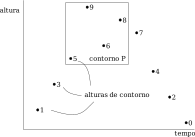
\includegraphics[scale=1.2]{cspace-5968}
  \end{figure}
}


\end{document}
